\section{Neural network implementation}
\subsection{Architecture}
A {\it mhcflurry} predictor consists of a embedding layer which transforms each amino acid to a learned vector representation, followed by a single hidden layer and finally a scalar output (figure \ref{architecture}). We map IC50 concentrations onto a regression target between 0.0 and 1.0 using the same scheme as NetMHC, $y = 1.0 - max(1.0, log_{50000}(IC50))$.

\begin{figure}[h]
\centering
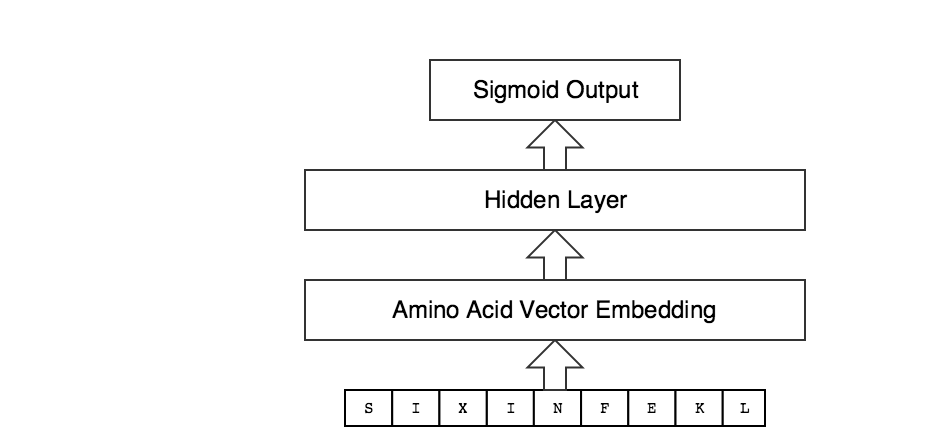
\includegraphics[scale=0.5]{figures/mhcflurry-gliffy-network.png}
\caption{Neural network architecture for predicting peptide-MHC affinities from fixed length amino acid sequences}
\label{fig:architecture}
\end{figure}

\subsection{Using a 9mer model on peptides of various lengths}
Like NetMHC\cite{lundegaard2008accurate}, the mhcflurry predictor assumes length-9 peptides and uses an averaging scheme to reduce non-9mer peptides to a 9mer prediction task. Each non-9mer is mapped into multiple 9mer query peptides, and the predicted affinity is taken to be the geometric mean of the predictions for the queries. For 8mers, the query peptides are generated by inserting a sentinel ``X'' at every position in the sequence. For peptides longer than 9 amino acids, 9mers are generated by removing consecutive stretches of residues at every position. This scheme is also used for training, with the affinity of each query peptide set equal to the measured affinity of the non-9mer peptide it was generated from, and its weight adjusted so each measurement receives equal contribution.

\section{Imputed training data}
For each allele, we train a mhcflurry model using the measured peptide affinities for the allele and the values imputed by MICE based on other alleles in the training set. As training progresses, we place decreasing weight on the imputed values, a strategy we refer to as "soft" dataset augmentation. The schedule used assigns each imputed observation at training epoch $i$ weight $1 / (1 + i)^2$.

\section{Random negative samples}
A randomly generated peptide is unlikely to bind a given MHC strongly, but a data acquisition bias toward strong binders in the training set can lead models to erroneously assign most peptides high affinity. As a form of regularization, we augment the training set at each epoch to include random peptides with affinity set to be maximally weak. The peptides are generated by drawing each amino acid uniformly at random. The number of random negative peptides is 20\% of the training size (without imputation). At each training epoch, a fresh set of random peptides are generated.

